\subsubsection{Thiết kế sơ đồ lớp}
Sơ đồ lớp thể hiện cấu trúc tĩnh và mối quan hệ giữa các thành phần cốt lõi của hệ thống TravelEZ:
\begin{itemize}
    \item \textbf{Định danh và Phân quyền:} Lớp trừu tượng \texttt{User} định nghĩa các thuộc tính nền tảng như \texttt{username}, \texttt{email}. Ba lớp kế thừa \texttt{Traveler}, \texttt{Provider}, và \texttt{Admin} thực thi các nghiệp vụ đặc thù cho từng vai trò người dùng.
    \item \textbf{Quản lý lộ trình:} Lớp \texttt{Itinerary} quản lý dữ liệu hành trình \(\texttt{budget}, \texttt{startDate}, \texttt{endDate}\) và tích hợp các phương thức AI xử lý dữ liệu động như \texttt{aiSuggestContent}. Mối quan hệ Composition giữa \texttt{Itinerary} và \texttt{ItineraryActivity} đảm bảo tính toàn vẹn của các hoạt động trong một lịch trình.
    \item \textbf{Quản lý Nội dung:} Các lớp \texttt{Review}, \texttt{Comment} và \texttt{BlogPost} kế thừa từ lớp \texttt{Content}, cho phép áp dụng đồng nhất các quy tắc kiểm duyệt qua \texttt{ViolatingKeyword}.
    \item \textbf{Kiểm duyệt và An toàn:} Hệ thống sử dụng \texttt{ContentReport} để tiếp nhận báo cáo và \texttt{ViolationRecord} để lưu vết vi phạm. Admin thực hiện kiểm duyệt tự động thông qua việc quản lý danh sách \texttt{ViolatingKeyword}.
    \item \textbf{Giao tiếp và Tiện ích:} Tính năng tương tác trực tiếp được thiết lập qua lớp \texttt{Conversation} và \texttt{Message}. Lớp \texttt{AiPromptHistory} lưu trữ lịch sử truy vấn để giám sát và tối ưu hóa chất lượng phản hồi từ hệ thống AI.
\end{itemize}
\begin{figure}[H]
    \centering
    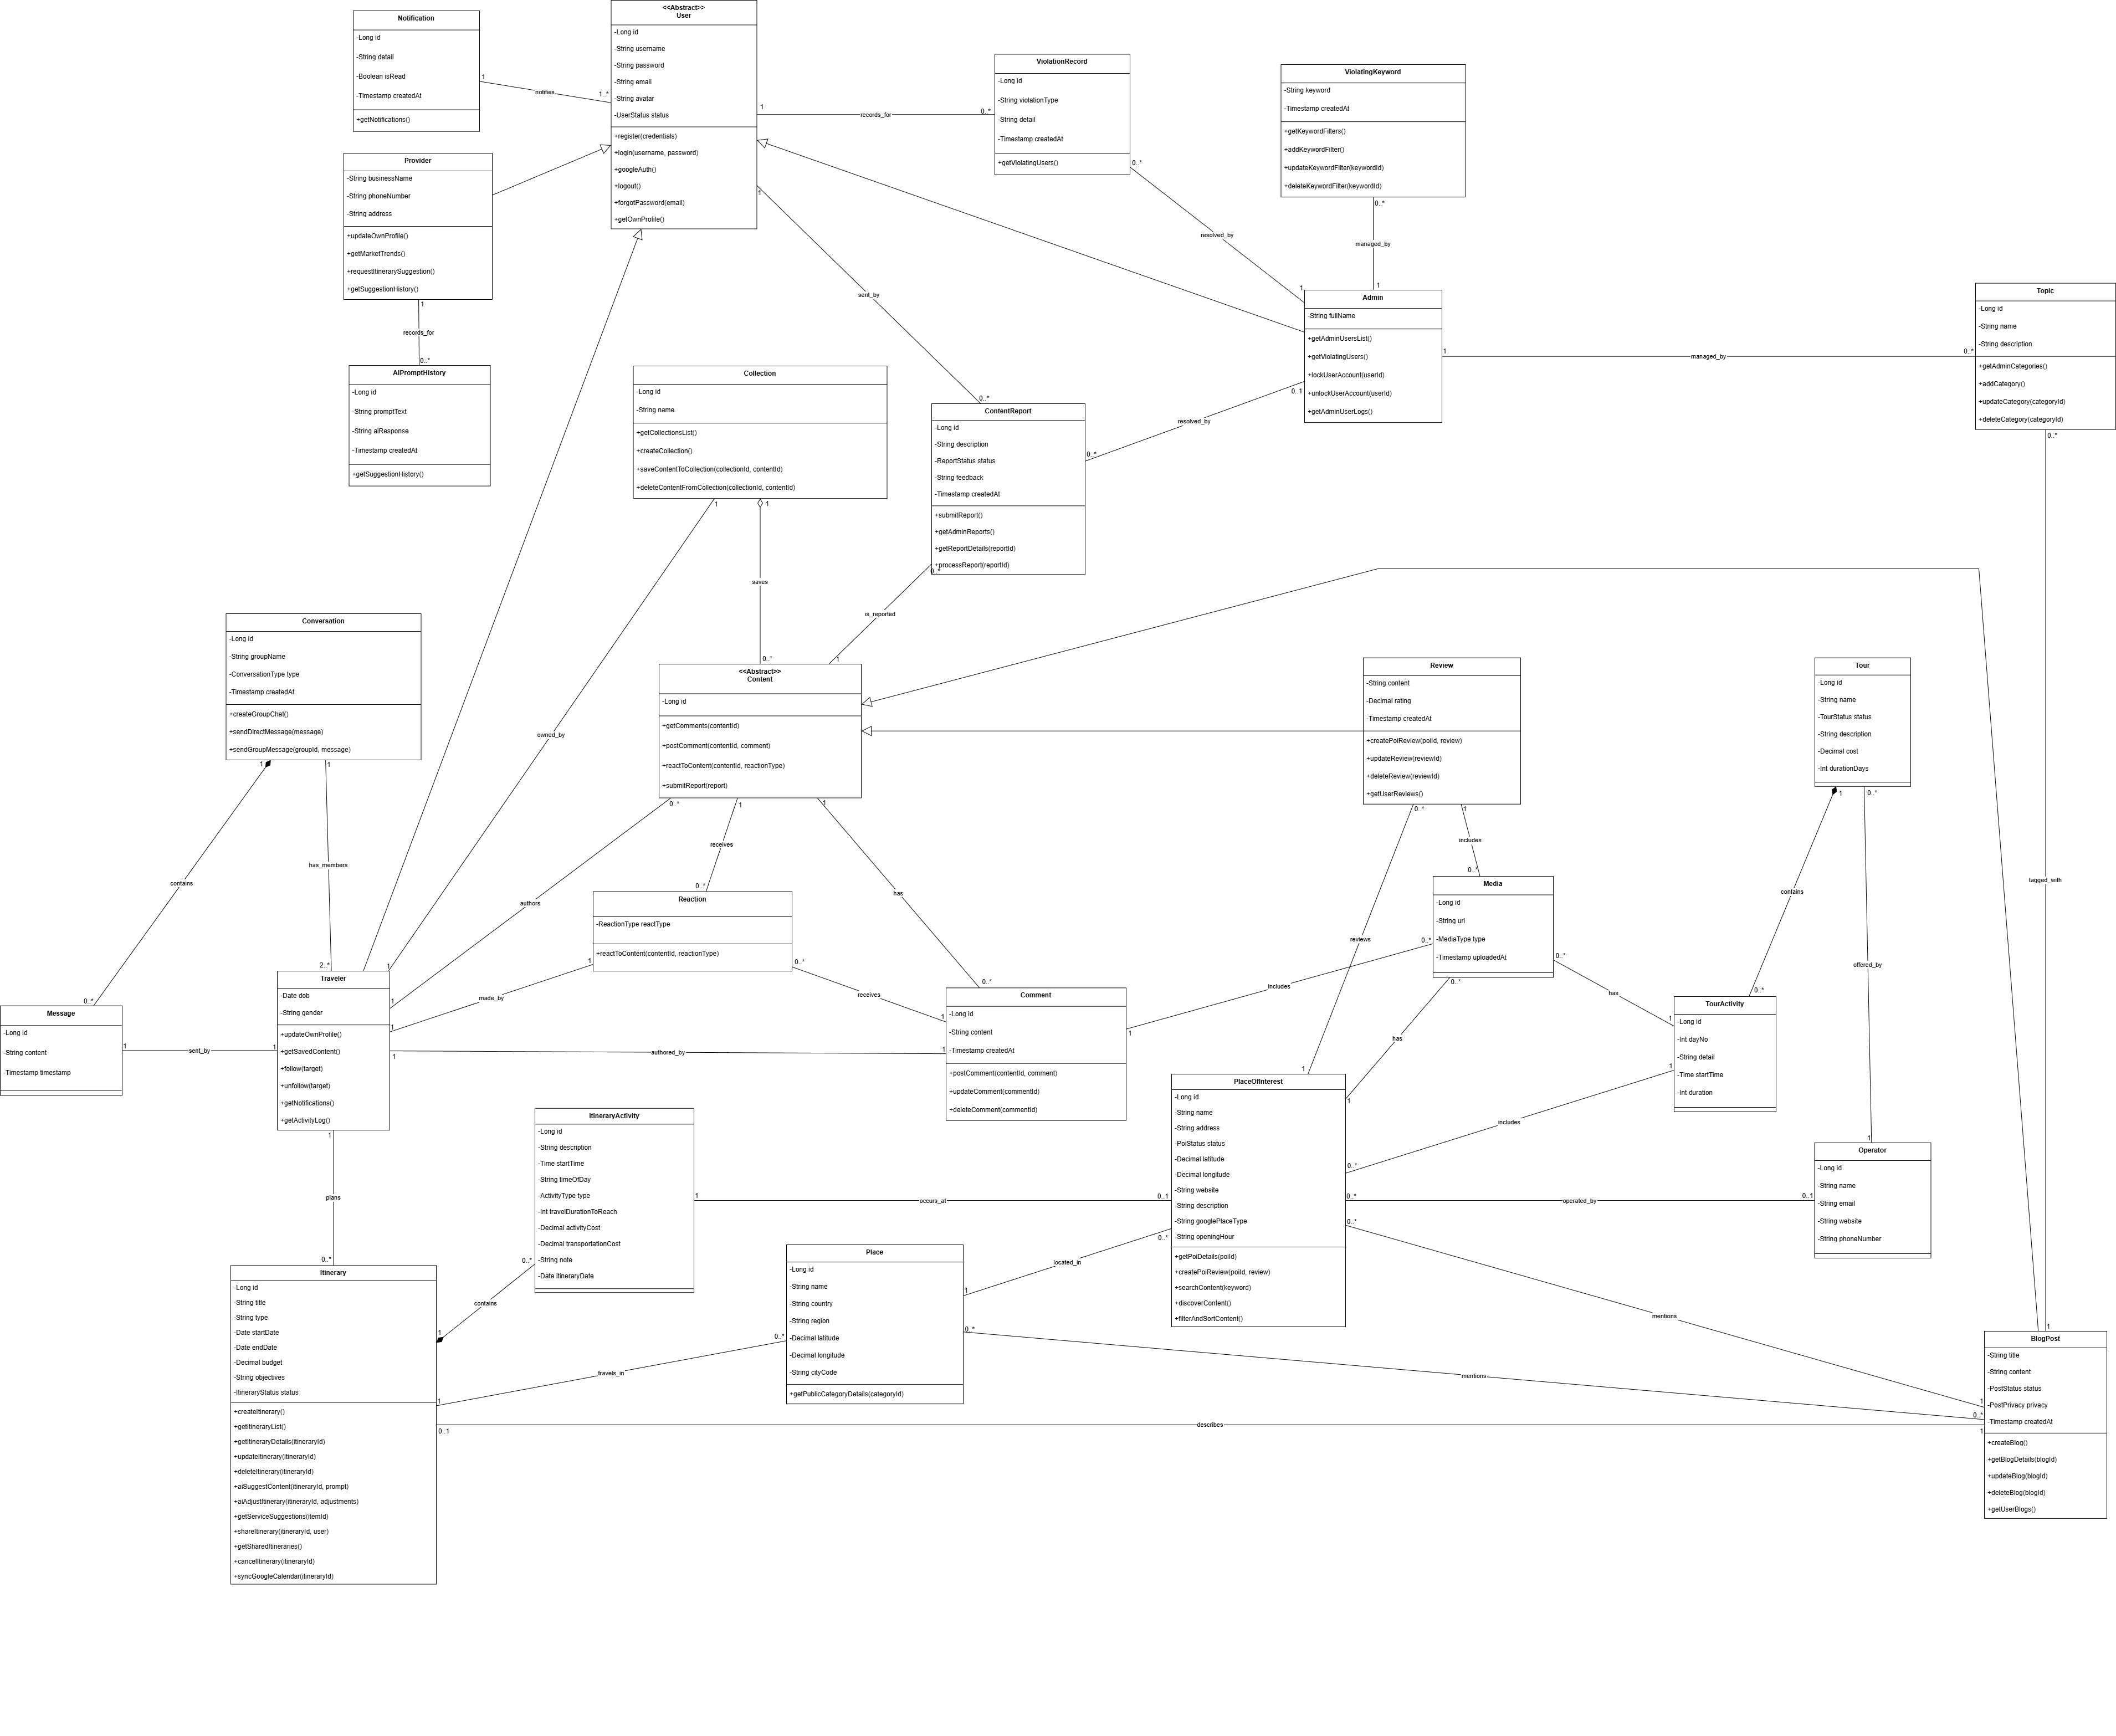
\includegraphics[width=\textwidth]{Images/7. System Design/ClassDiagram.png}
    \caption{Sơ đồ lớp của hệ thống TravelEZ}
    \label{fig:class-diagram}
\end{figure}